\section{Software}\label{Software}
\subsection{Prerequisites}
\begin{itemize}
\item Node.js (Javascript runtime)
\item Angular
\item IDE (Visual Studio Code)
\item Datenbank (MariaDb)
\end{itemize}

\subsection{Frontend - SmartMirrorWeb}
\begin{figure}[h]
\centering
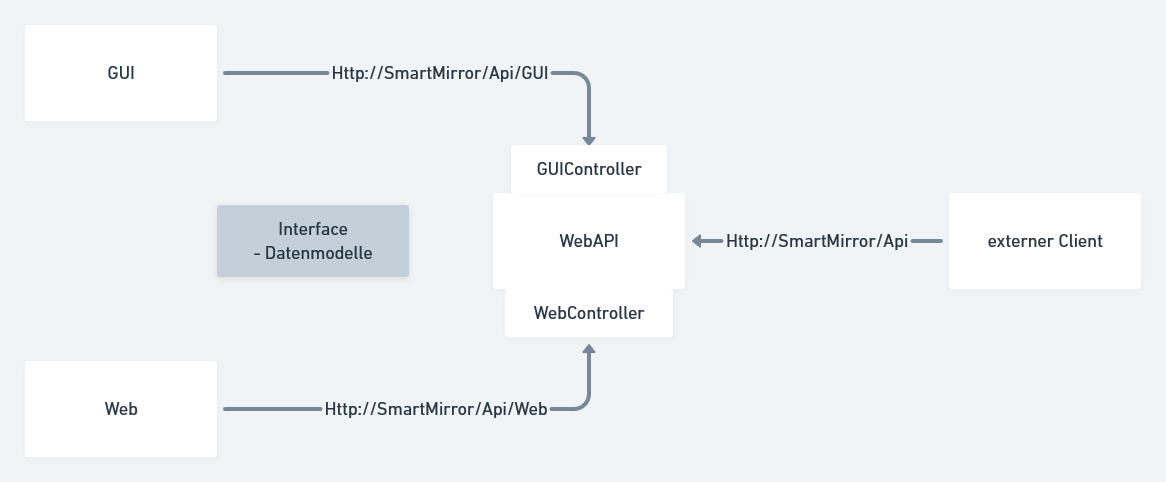
\includegraphics[width=120mm]{pictures/Frontend2.png}
\caption{konzeptioneller Aufbau der Software-Komponenten}
\end{figure}
Wir haben unser Frontend mithilfe von Angular 9 entwickelt. Für uns war dies eine Neue Erfahrung, da wir noch nie zuvor damit gearbeitet haben. Das Frontend soll sich lediglich um die Anzeige der Daten kümmern und folgende Funktionen übernehmen:
\begin{itemize}
\item Daten vom Backend (SmartMirror.WebApi) anfragen
\begin{itemize}
\item alle möglichen Dienste (Widgets)
\item vom User angemeldeten Dienste
\end{itemize}
\item Daten senden
\begin{itemize}
\item Dienst aktivieren/ deaktivieren
\item Benutzereingaben zur Erstellung eines neuen Benutzers
\end{itemize}
\item User zur Anmeldung von weiteren externen Diensten, zur jeweiligen Website weiterleiten\footnote{zum Beispiel: wenn der User den neuen Dienst Google Kalender für sich registrieren möchte, muss er sich auf der Website von Google Kalender anmelden um sich zu zertifizieren. Diese sendet dann die zur Authentifizierung notwendigen Credentials, welche vom Backend gespeichert werden müssen }
\end{itemize} 
\subsection{Backend - SmartMirror.WebApi}
Das Backend besteht aus einer eigens Entwickelten Web API, welche zum einen die Anfragen und Daten vom Frontend (SmartMirror.Web) entgegennimmt und bearbeitet, und zum anderen den Datenaustausch mit der eigenen Datenbank und Kommunikation mit den externen API kommuniziert.\\\
Das Backend besteht zum einen Client-Server. Zum einen stellt er als Server eine eigene API dar, welche vom Frontend genutzt wird. Zum anderen fungiert dieser auch als Client und nutzt die externen API Schnittstellen von Drittanbietern. Besitzt dieser eine extra Komponente, welche auf die interne Datenbank zugreift\\\
\subsection{GUI - SmartMirror.GUI}
Die digitale Darstellung, aller Module die zuvor auf der Website konfiguriert wurden, auf dem Spiegel wird durch unsere eigene GUI - Applikation ("Graphical User Interface") ausgeführt. Diese wurde in der Programmiersprache C# geschrieben, welches uns die simple Erstellung einer Desktop Applikation ermöglichte und uns zudem auch aus dem Studium bekannt ist. 
Das Ziel war es ein kompatibles System aufzubauen. Deshalb sollte die Applikation Betriebssystem unabhänig sein, dass heißt es sollte auf jedem Betriebssysteme mit gleicher Performance laufen können. Die Wahl mit C# und .NET hat diese Entscheidung für uns schwer getan, da das .NET Framework und .NET Core ihre Windows Desktop Applikationen eher für "Windows-only", von Microsoft, konzipiert wurden. Das Betriebssystem auf dem Raspberry Pi ist "Raspbian" und basiert auf den Linux Kernel. Das Problem konnten wir mit einigen zusätzlichen Erweiterungen beheben. Um eine Kompatibilität unserer GUI-Applikation mit Linux herstellen zu können, mussten wir zusätzliche Framework Installationen auf den Raspberry Pi durchführen. 
Eine Lösung wäre das "Avalonia-Framework", welches die Entwicklung von Desktop Applikationen unter .NET Core in der Programmiersprache C# ermöglicht. Damit könnte man schon von Beginn an die Applikation für Linux entwickeln. Diese Lösungsmöglichkeit wird auch auf unser GUI-Projekt ("SmartMirror.GUI", im GitHub Repository zu finden) angewandt. 
Für Universelle Windows Systeme haben wir die "SmartMirror.GUI_UWP" entwickelt. Die Benutzeroberfläche ist identisch wie die SmartMirror.GUI, die selben Funktionalitäten werden unterstützt nur für verschiedene Systeme.


\paragraph{Server Funktion}

\paragraph{Kommunikation zur Datenbank}


\subsection{Komponenten}\label{Komponenten}
\subsubsection{Clients}\label{Clients}
Da der Smart Mirror möglichst viele externe Features verbinden soll, muss die Schnittstelle zu diesen gut strukturiert werden. Daher haben wir uns dazu entschieden, dass jede externe Kommunikation ihre eigene Komponente bekommet, welche bestimmte Standards (Interfaces) bedient
Die Clients, wobei jeder auf eine spezifische externe API ausgreichtet ist, übernehemen die Kommunikationion zu diesen. Sie kümmern sich um die Authorisierung, Datenabfrage und stellen der WebAPI bestimmte einheitliche Funktionen bereit. Jeder Client muss diese implementieren. Zusätzlich ist der Aufbau der Daten, die zwischen der WebAPI und den Clients übertragen werden, vereinheitlicht und fest definiert. Diese vereinheitlichten Funktionen und Datenmodelle sind in von uns definierten Interfaces beschrieben. Ein Client muss sich an die vorgebenen Funktionen und Datenmodelle halten. Dabei haben wir geguckt, welche Funktionen essentiell wichtig für die Kommunikation sind und wie wir die Daten optimal strukturieren können. (einige Funktionen um nicht zu sehr ins Detail zu gehen zb.: getData(Options):Data, welche Daten von der API und den Bedingungen abfragt; getOptions():Options, welche die Verfügbaren Optionen abfragt; setToken(string):bool, welche den Authorisierungstoken für den jeweiligen Client setzt). Wenn eine neue externe API bereitgestellt werden soll, muss lediglich ein Client programmiert werden, welcher die vorgeschriebenen Funktionen und Datenmodelle implementiert (Interfaces) und die jeweiligen Http-Requests für die API beinhaltet. So kann zu jeder API unter berücksichtigung der Standards ein passender Client programmiert werden. Anschließend muss dieser nur noch der WebAPI bekannt gemacht werden, indem der Client in eine interne Liste von allen möglichen externen Diensten eingetragen wird.\\\
\subsubsection{WebAPI}
\begin{figure}[h]
\centering
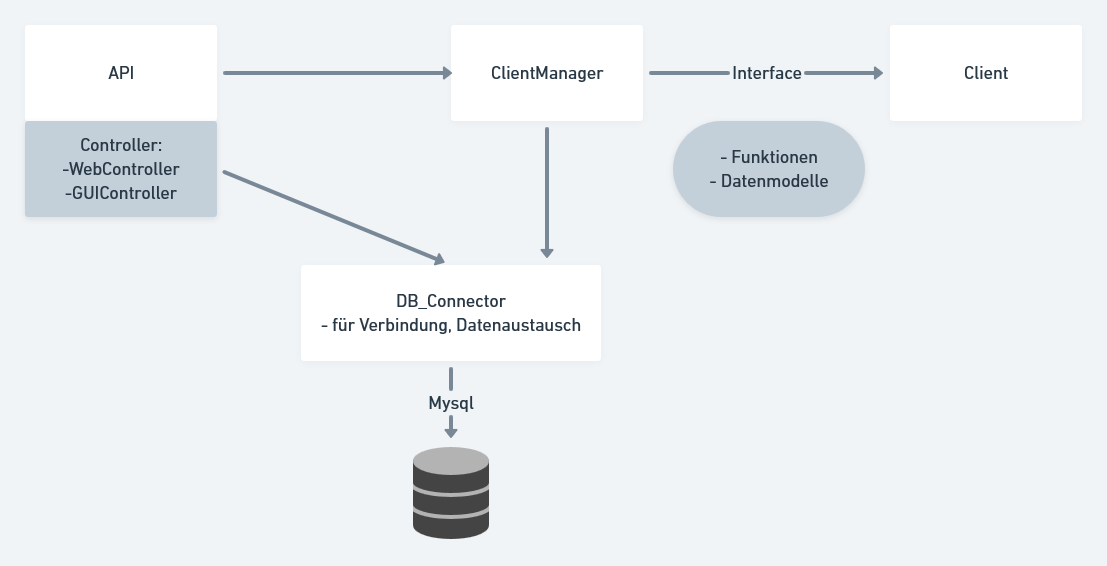
\includegraphics[width=120mm]{pictures/WebAPI.png}
\caption{konzeptioneller Aufbau der Software-Komponenten}
\end{figure}
\subsubsection{Database}
\begin{figure}[h]
\centering
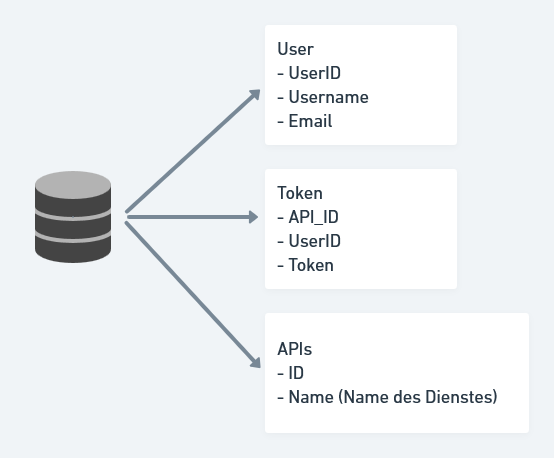
\includegraphics[width=80mm]{pictures/Database.png}
\caption{konzeptioneller Aufbau der Software-Komponenten}
\end{figure}


